\documentclass[]{article}
\usepackage{lmodern}
\usepackage{amssymb,amsmath}
\usepackage{ifxetex,ifluatex}
\usepackage{fixltx2e} % provides \textsubscript
\ifnum 0\ifxetex 1\fi\ifluatex 1\fi=0 % if pdftex
  \usepackage[T1]{fontenc}
  \usepackage[utf8]{inputenc}
\else % if luatex or xelatex
  \ifxetex
    \usepackage{mathspec}
    \usepackage{xltxtra,xunicode}
  \else
    \usepackage{fontspec}
  \fi
  \defaultfontfeatures{Mapping=tex-text,Scale=MatchLowercase}
  \newcommand{\euro}{€}
\fi
% use upquote if available, for straight quotes in verbatim environments
\IfFileExists{upquote.sty}{\usepackage{upquote}}{}
% use microtype if available
\IfFileExists{microtype.sty}{%
\usepackage{microtype}
\UseMicrotypeSet[protrusion]{basicmath} % disable protrusion for tt fonts
}{}
\usepackage[margin=1in]{geometry}
\usepackage{color}
\usepackage{fancyvrb}
\newcommand{\VerbBar}{|}
\newcommand{\VERB}{\Verb[commandchars=\\\{\}]}
\DefineVerbatimEnvironment{Highlighting}{Verbatim}{commandchars=\\\{\}}
% Add ',fontsize=\small' for more characters per line
\usepackage{framed}
\definecolor{shadecolor}{RGB}{248,248,248}
\newenvironment{Shaded}{\begin{snugshade}}{\end{snugshade}}
\newcommand{\KeywordTok}[1]{\textcolor[rgb]{0.13,0.29,0.53}{\textbf{{#1}}}}
\newcommand{\DataTypeTok}[1]{\textcolor[rgb]{0.13,0.29,0.53}{{#1}}}
\newcommand{\DecValTok}[1]{\textcolor[rgb]{0.00,0.00,0.81}{{#1}}}
\newcommand{\BaseNTok}[1]{\textcolor[rgb]{0.00,0.00,0.81}{{#1}}}
\newcommand{\FloatTok}[1]{\textcolor[rgb]{0.00,0.00,0.81}{{#1}}}
\newcommand{\CharTok}[1]{\textcolor[rgb]{0.31,0.60,0.02}{{#1}}}
\newcommand{\StringTok}[1]{\textcolor[rgb]{0.31,0.60,0.02}{{#1}}}
\newcommand{\CommentTok}[1]{\textcolor[rgb]{0.56,0.35,0.01}{\textit{{#1}}}}
\newcommand{\OtherTok}[1]{\textcolor[rgb]{0.56,0.35,0.01}{{#1}}}
\newcommand{\AlertTok}[1]{\textcolor[rgb]{0.94,0.16,0.16}{{#1}}}
\newcommand{\FunctionTok}[1]{\textcolor[rgb]{0.00,0.00,0.00}{{#1}}}
\newcommand{\RegionMarkerTok}[1]{{#1}}
\newcommand{\ErrorTok}[1]{\textbf{{#1}}}
\newcommand{\NormalTok}[1]{{#1}}
\usepackage{graphicx}
\makeatletter
\def\maxwidth{\ifdim\Gin@nat@width>\linewidth\linewidth\else\Gin@nat@width\fi}
\def\maxheight{\ifdim\Gin@nat@height>\textheight\textheight\else\Gin@nat@height\fi}
\makeatother
% Scale images if necessary, so that they will not overflow the page
% margins by default, and it is still possible to overwrite the defaults
% using explicit options in \includegraphics[width, height, ...]{}
\setkeys{Gin}{width=\maxwidth,height=\maxheight,keepaspectratio}
\ifxetex
  \usepackage[setpagesize=false, % page size defined by xetex
              unicode=false, % unicode breaks when used with xetex
              xetex]{hyperref}
\else
  \usepackage[unicode=true]{hyperref}
\fi
\hypersetup{breaklinks=true,
            bookmarks=true,
            pdfauthor={Henry Scharf, edited to snowfall by John Tipton},
            pdftitle={moving from for to snowfall},
            colorlinks=true,
            citecolor=blue,
            urlcolor=blue,
            linkcolor=magenta,
            pdfborder={0 0 0}}
\urlstyle{same}  % don't use monospace font for urls
\setlength{\parindent}{0pt}
\setlength{\parskip}{6pt plus 2pt minus 1pt}
\setlength{\emergencystretch}{3em}  % prevent overfull lines
\setcounter{secnumdepth}{0}

%%% Use protect on footnotes to avoid problems with footnotes in titles
\let\rmarkdownfootnote\footnote%
\def\footnote{\protect\rmarkdownfootnote}

%%% Change title format to be more compact
\usepackage{titling}
\setlength{\droptitle}{-2em}
  \title{moving from for to snowfall}
  \pretitle{\vspace{\droptitle}\centering\huge}
  \posttitle{\par}
  \author{Henry Scharf, edited to snowfall by John Tipton}
  \preauthor{\centering\large\emph}
  \postauthor{\par}
  \predate{\centering\large\emph}
  \postdate{\par}
  \date{May 6, 2014}




\begin{document}

\maketitle


{
\hypersetup{linkcolor=black}
\setcounter{tocdepth}{2}
\tableofcontents
}
\section{why?}\label{why}

\subsection{embarassingly parallel
tasks}\label{embarassingly-parallel-tasks}

These are computational tasks which involve many separate, independently
executable calculations. Some common statistical examples of
embarassingly {\textbf{parallel}} processes:

\begin{itemize}
\itemsep1pt\parskip0pt\parsep0pt
\item
  bootstrapping
\item
  cross-validation
\item
  simulating independent random variables (\texttt{dorng})
\end{itemize}

In contrast, some sequential or {\textbf{non-parallel}} processes:

\begin{itemize}
\itemsep1pt\parskip0pt\parsep0pt
\item
  MCMC algorithms
\item
  several types of model selection (e.g.: \texttt{step()} or the LARS
  algorithm for LASSO)
\end{itemize}

\texttt{for} loops that do not explicitly involve dependent calculations
are wasteful if we have multiple processors available. Perhaps even
worse, the time cost of using such an approach can put some useful
statistical tools beyond our reach!

\subsection{options}\label{options}

\begin{itemize}
\itemsep1pt\parskip0pt\parsep0pt
\item
  Changing from a for loop to one of the \texttt{apply()} functions can
  help, but still doesn't use multiple processors.
\item
  Use the \texttt{parallel} package.
\item
  Don't use R.
\item
  Use the \texttt{snowfall} package! {[}@snowfall{]}
\end{itemize}

\subsection{why snowfall?}\label{why-snowfall}

We would like to find a way to make use of our whole computer, and make
valuable tasks like bootstrapping available, but without having to
invest large amounts of time in learning new programming languages.
Enter \texttt{snowfall}, which keeps the structure of a for loop, but
allows us to drop two key assumptions:

\begin{itemize}
\itemsep1pt\parskip0pt\parsep0pt
\item
  sequentiality
\item
  single processor architecture
\end{itemize}

{\textbf{Our goal}}: We will begin with a simple chunk of R code
involving a for loop and transform it into a \texttt{snowfall} loop.
Along the way, we'll take a look at the equivalent computation done with
an \texttt{apply()} function, and see that using \texttt{snowfall} and
multiple processors outperforms this.

\section{example: data and research
question}\label{example-data-and-research-question}

We are going to look at data from the New York City bikeshare program
\href{https://www.citibikenyc.com/}{Citibike}.

\begin{itemize}
\itemsep1pt\parskip0pt\parsep0pt
\item
  7 busiest locations from May 2014
\item
  response: \# of arrivals each hour of every day in the month
\item
  covariates: hour of the day and whether the day is a weekend
\end{itemize}

One of the costliest parts of operating a bike share program comes from
the finiteness of the bicycle stations. A station can only hold so many
bicycles, and a full (empty) station means customers cannot drop off
(pick up) a bike. Thus, managers are forced to use trucks to manually
redistribute bicycles.

We want to find a model which can offer good prediction, with the hope
that this will inform our plans for future station locations/sizes. For
this example, we start with a few plausible models and use K-fold cross
validation to decide which one to use.

\subsection{locations of our 7 sites}\label{locations-of-our-7-sites}

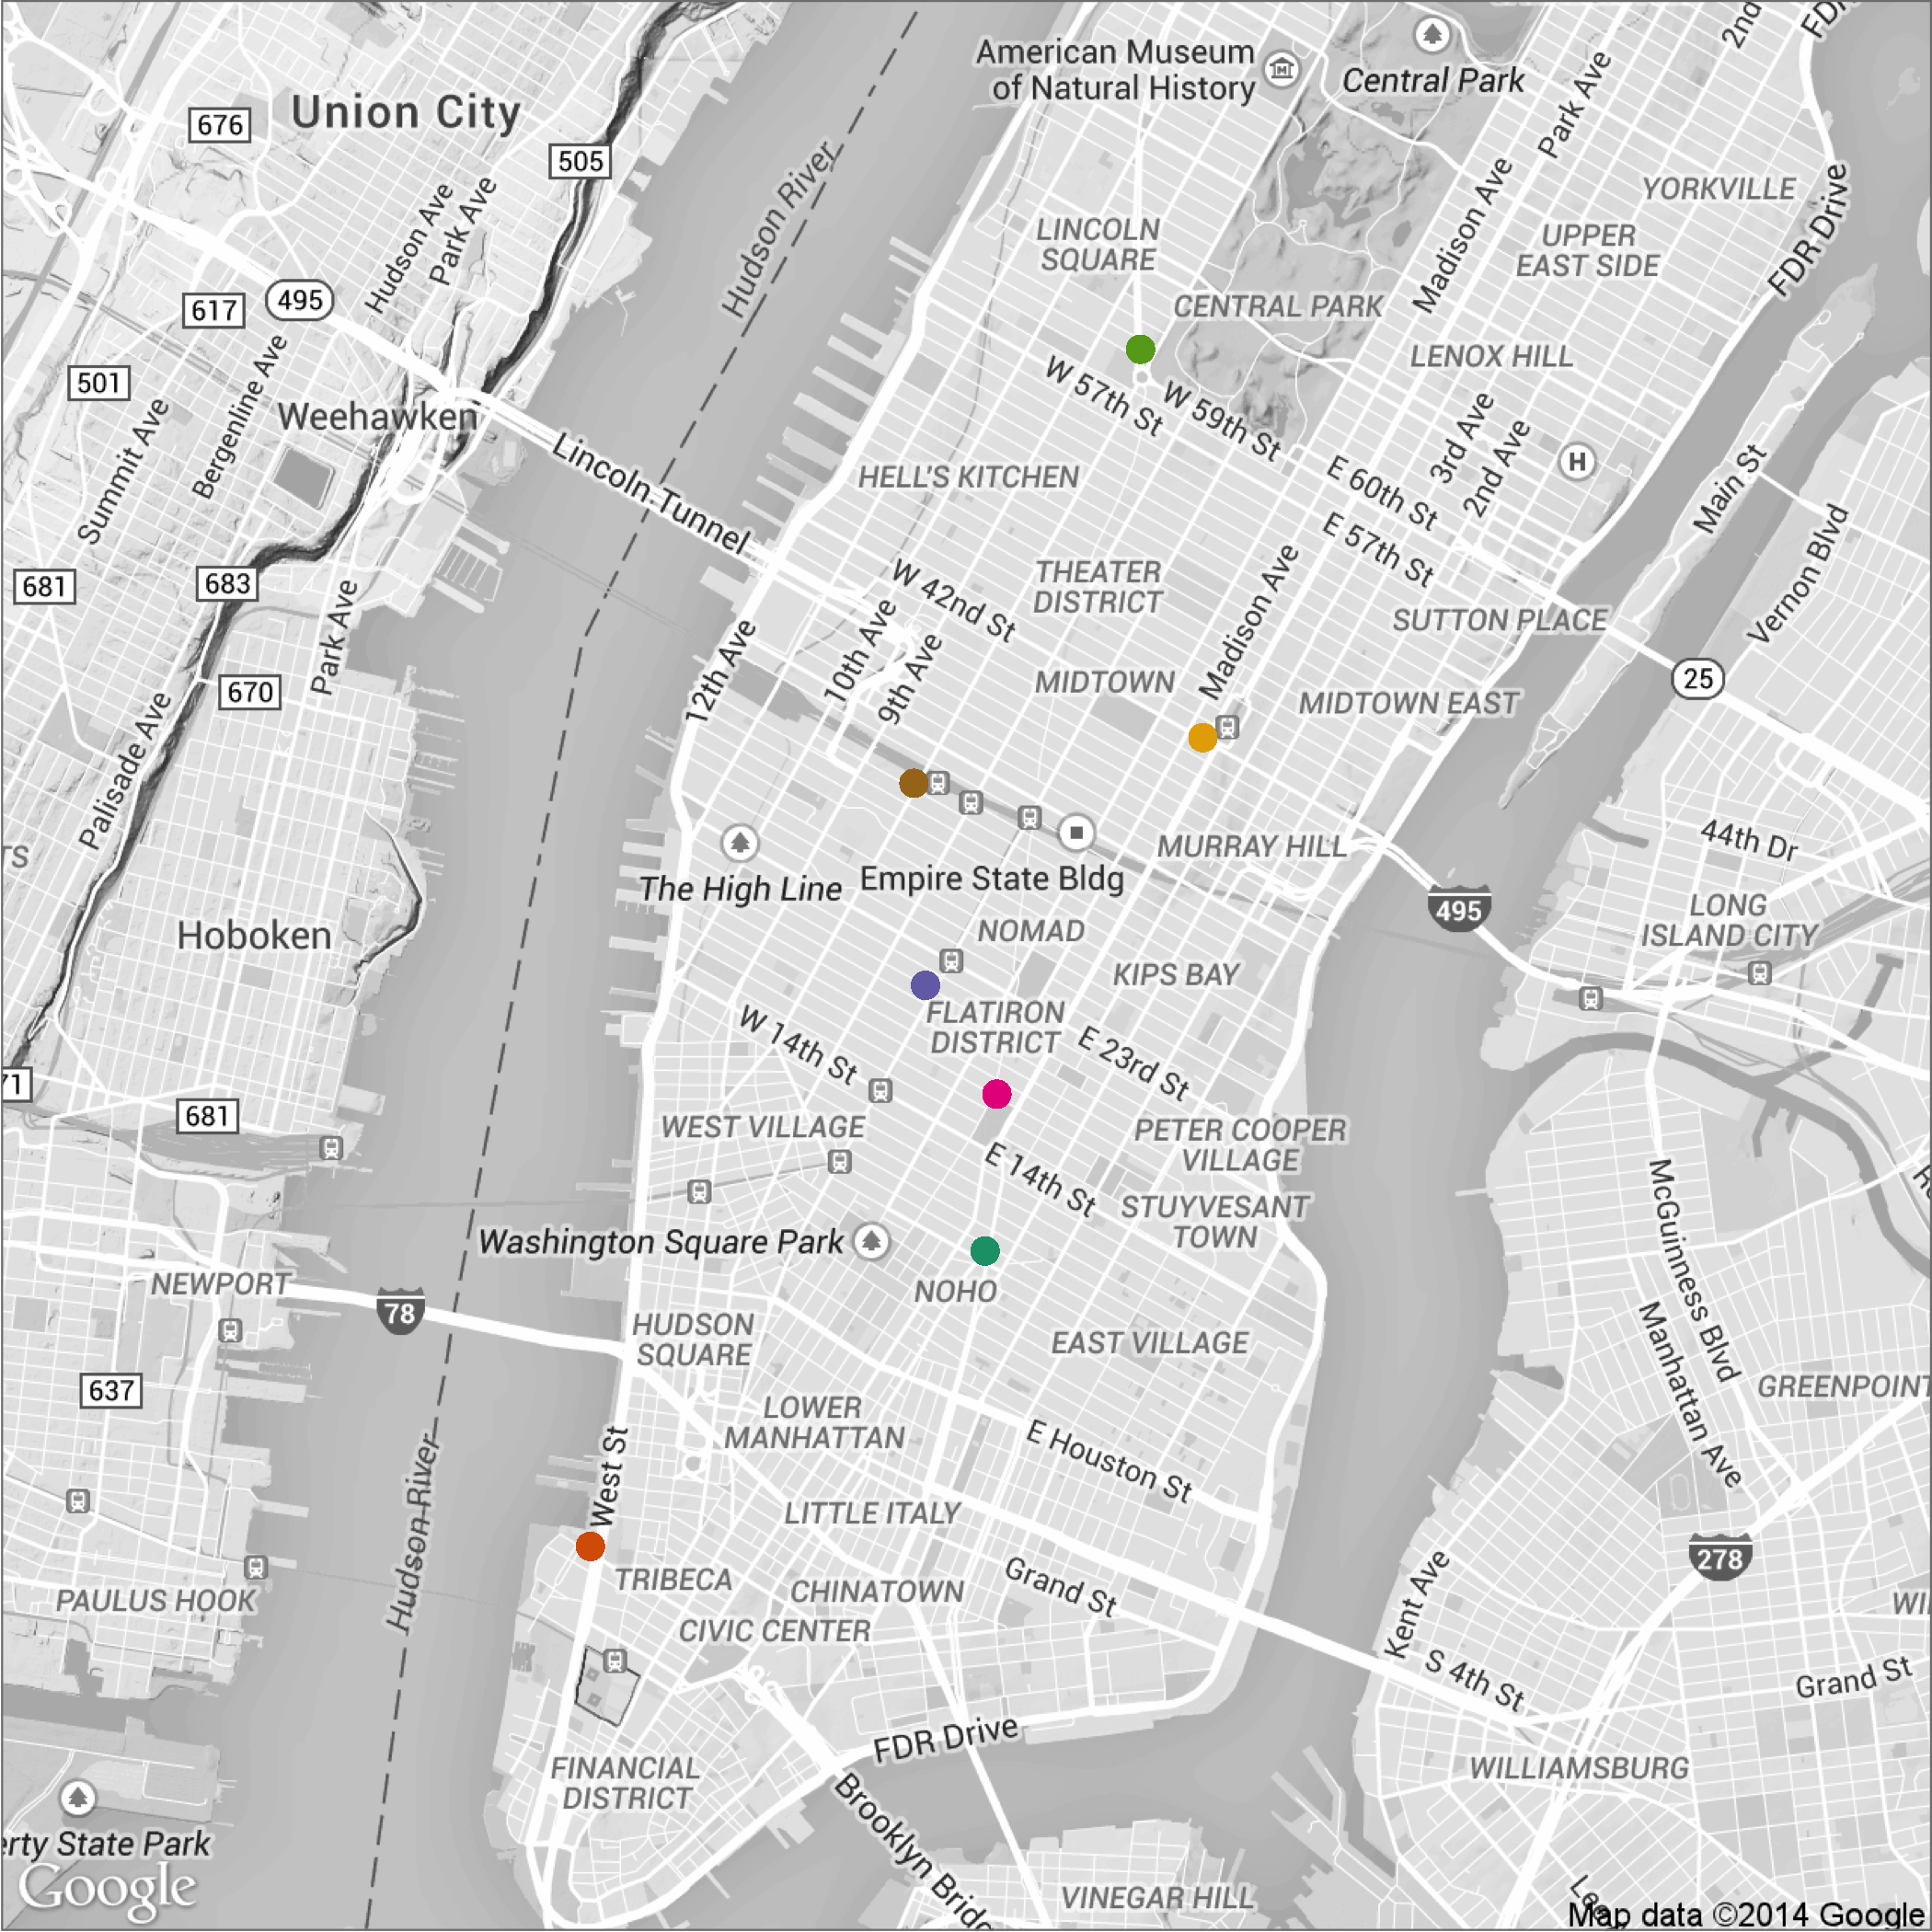
\includegraphics{./fig/map_top7.png}

\begin{center}\rule{0.5\linewidth}{\linethickness}\end{center}

\subsection{data}\label{data}

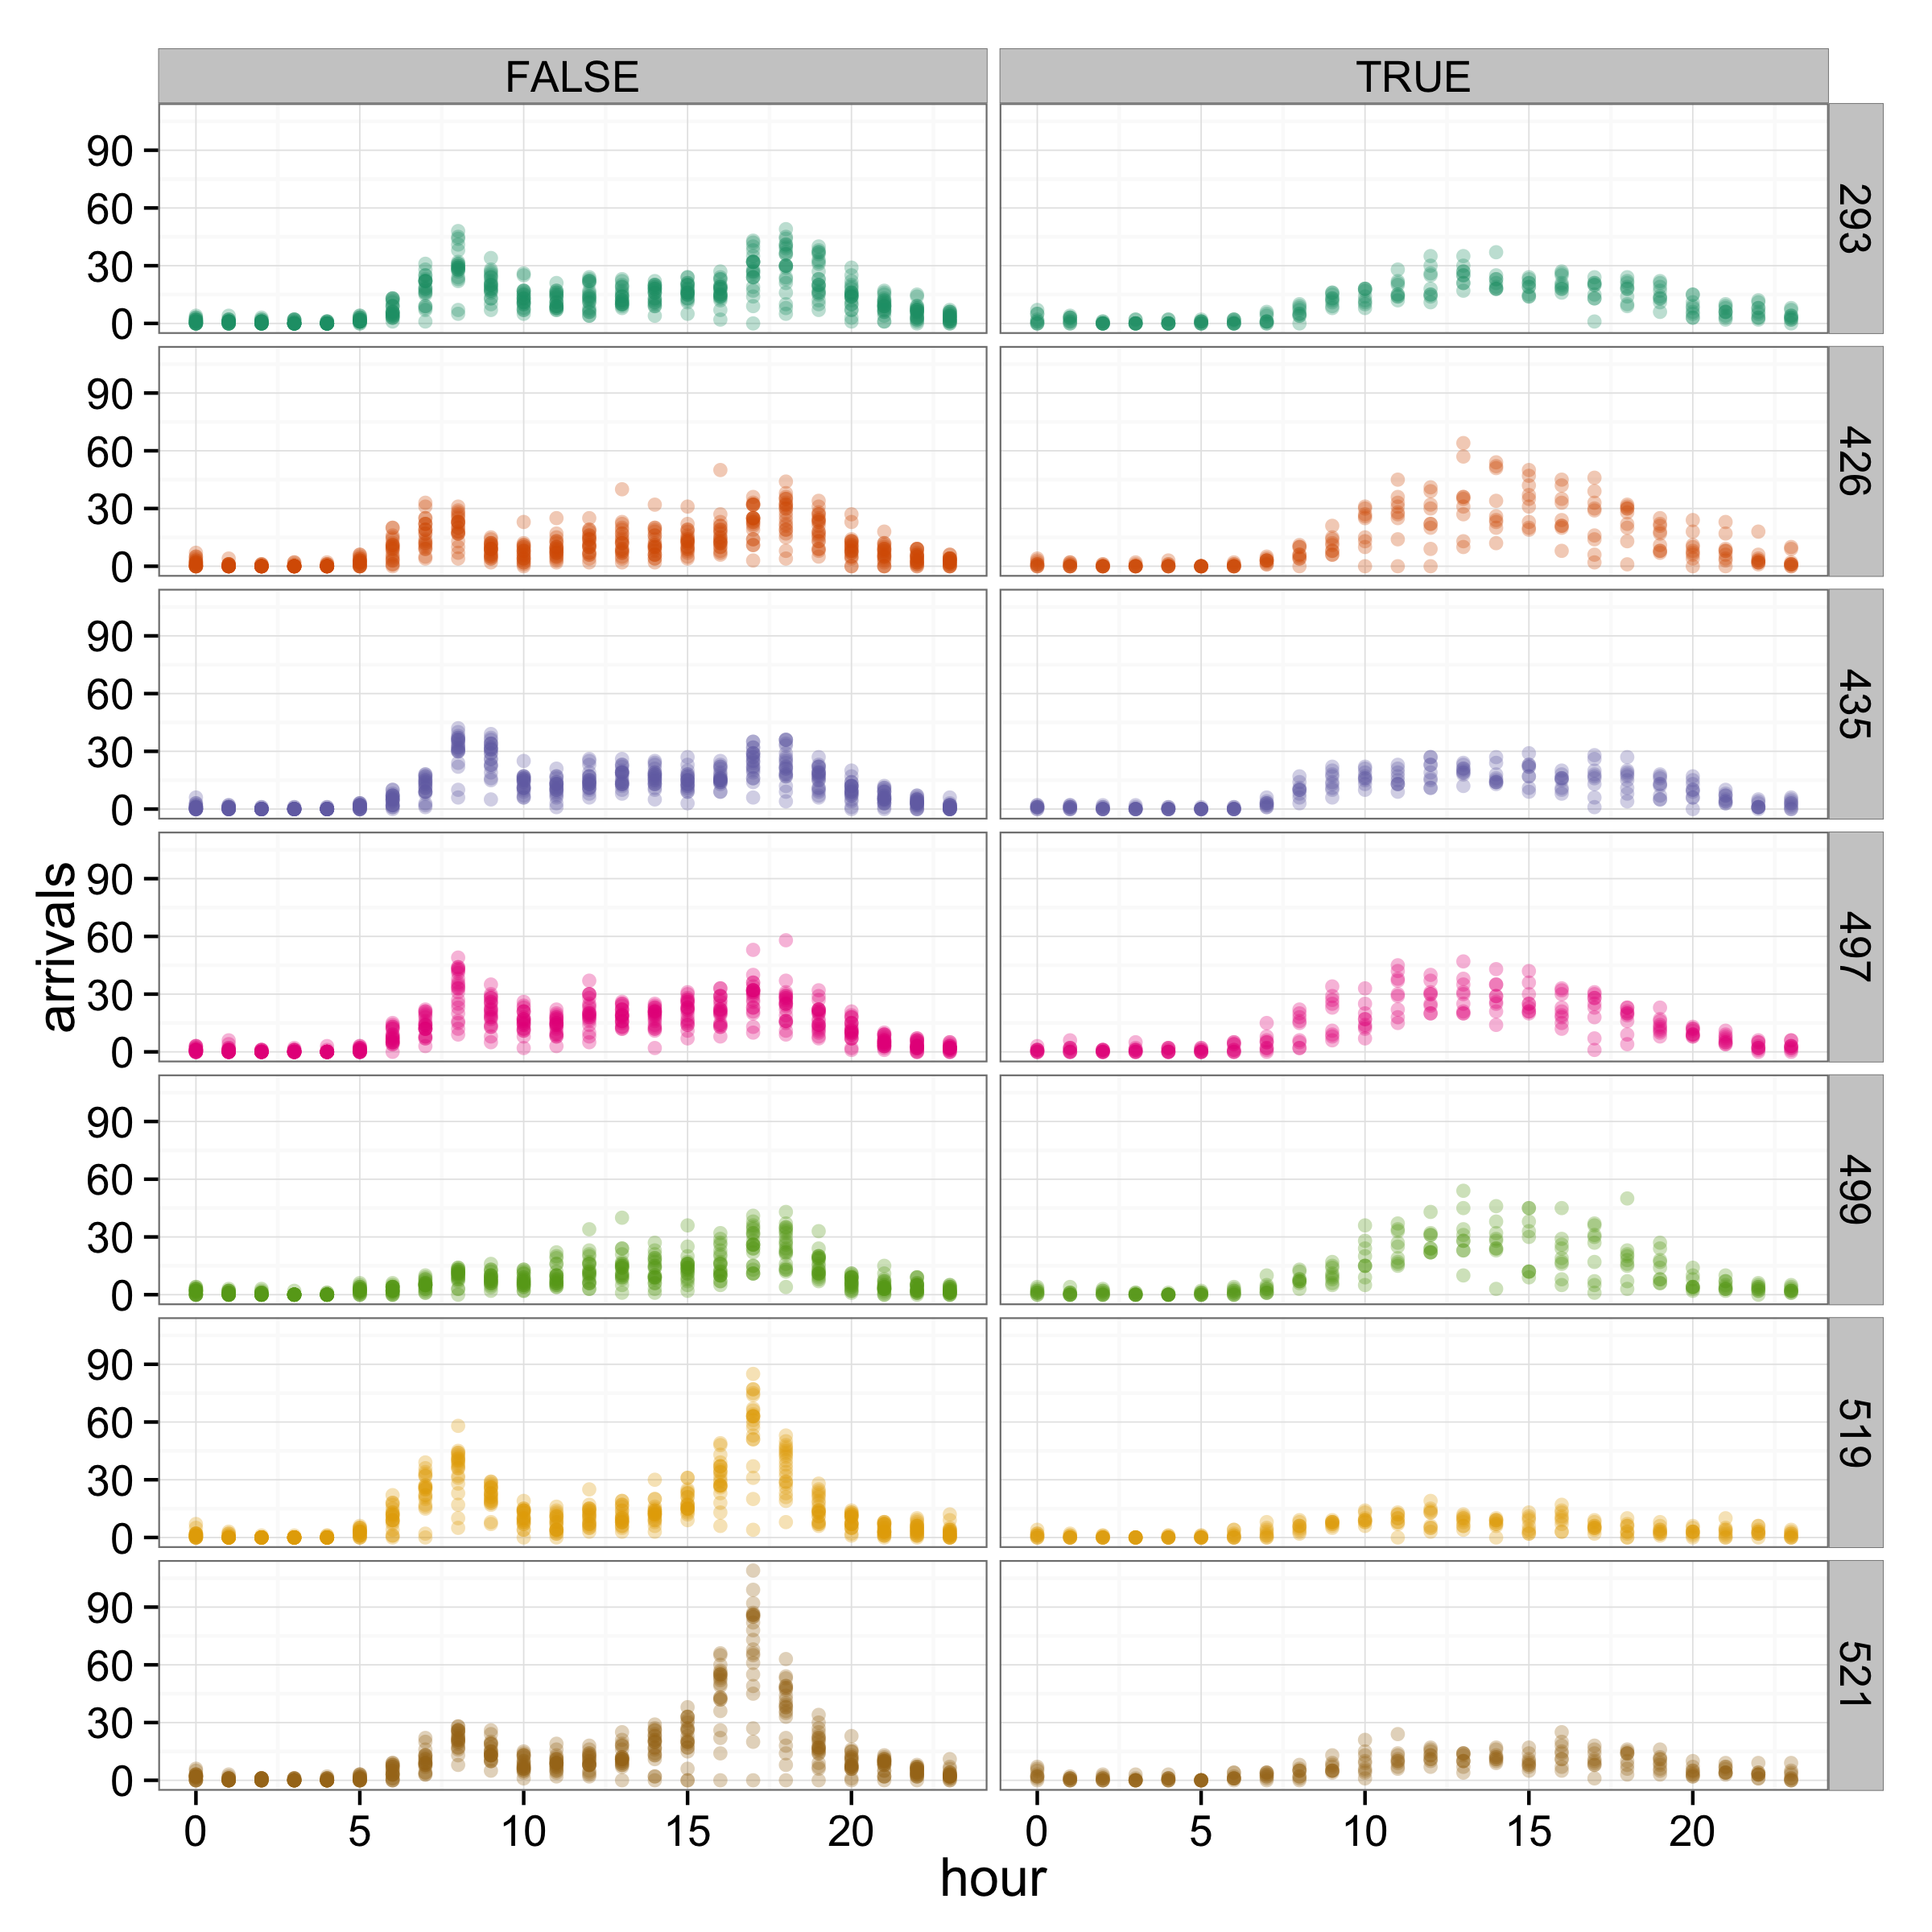
\includegraphics{./fig/top7_average_day.png}

\begin{center}\rule{0.5\linewidth}{\linethickness}\end{center}

\section{fitting GLMs and extracting prediction
error}\label{fitting-glms-and-extracting-prediction-error}

We are considering three increasingly complex models of the arrival
behavior. In order to compare three candidate models' prediction error,
we'll use K-fold cross validation, where we use the same folds for all
three models.

First, we the load the data and make our K-fold test sets (and
implicitly, our training sets):

\begin{Shaded}
\begin{Highlighting}[]
\KeywordTok{load}\NormalTok{(}\KeywordTok{url}\NormalTok{(}\StringTok{"http://www.stat.colostate.edu/~scharfh/CSP_parallel/data/arrivals_subset.RData"}\NormalTok{))}
\NormalTok{K <-}\StringTok{ }\DecValTok{50}
\NormalTok{N <-}\StringTok{ }\KeywordTok{dim}\NormalTok{(arrivals.sub)[}\DecValTok{1}\NormalTok{]}

\NormalTok{## for convenience kill off 8 observations (we have 5208) and make cv test sets}
\KeywordTok{set.seed}\NormalTok{(}\DecValTok{1985}\NormalTok{)}
\NormalTok{discarded <-}\StringTok{ }\KeywordTok{sample}\NormalTok{(}\DecValTok{1}\NormalTok{:N, }\DataTypeTok{size =} \DecValTok{8}\NormalTok{)}
\NormalTok{cv.test.sets <-}\StringTok{ }\KeywordTok{matrix}\NormalTok{(}\KeywordTok{sample}\NormalTok{((}\DecValTok{1}\NormalTok{:N)[-discarded], }\DataTypeTok{size =} \NormalTok{N -}\StringTok{ }\DecValTok{8}\NormalTok{), }\DataTypeTok{ncol =} \NormalTok{K)}
\end{Highlighting}
\end{Shaded}

Next, we build a function to fit the data to the training sets and
extract the corresponding estimate of prediciton error. This should
still be familiar code, no new packages yet.

\begin{Shaded}
\begin{Highlighting}[]
\KeywordTok{library}\NormalTok{(splines)}
\NormalTok{lq.loss <-}\StringTok{ }\NormalTok{function(y, y.hat, }\DataTypeTok{q =} \DecValTok{1}\NormalTok{) \{(}\KeywordTok{abs}\NormalTok{(y -}\StringTok{ }\NormalTok{y.hat))^q\}}
\NormalTok{get.errs <-}\StringTok{ }\NormalTok{function(}\DataTypeTok{test.set =} \OtherTok{NULL}\NormalTok{,}
                     \DataTypeTok{discarded =} \OtherTok{NULL}\NormalTok{,}
                     \DataTypeTok{q =} \DecValTok{1}\NormalTok{) \{}
    \NormalTok{sml.glm <-}\StringTok{ }\KeywordTok{glm}\NormalTok{(arrivals ~}
\StringTok{                   }\KeywordTok{bs}\NormalTok{(hour, }\DataTypeTok{degree =} \DecValTok{4}\NormalTok{)}
                   \NormalTok{+}\StringTok{ }\NormalTok{weekend}
                   \NormalTok{+}\StringTok{ }\KeywordTok{as.factor}\NormalTok{(id),}
                   \DataTypeTok{data =} \NormalTok{arrivals.sub[-}\KeywordTok{c}\NormalTok{(discarded, test.set), ],}
                   \DataTypeTok{family =} \StringTok{"poisson"}\NormalTok{)}
    \NormalTok{med.glm <-}\StringTok{ }\KeywordTok{glm}\NormalTok{(arrivals ~}
\StringTok{                   }\KeywordTok{bs}\NormalTok{(hour, }\DataTypeTok{degree =} \DecValTok{4}\NormalTok{)*weekend}
                   \NormalTok{+}\StringTok{ }\KeywordTok{as.factor}\NormalTok{(id),}
                   \DataTypeTok{data =} \NormalTok{arrivals.sub[-}\KeywordTok{c}\NormalTok{(discarded, test.set), ],}
                   \DataTypeTok{family =} \StringTok{"poisson"}\NormalTok{)}
    \NormalTok{big.glm <-}\StringTok{ }\KeywordTok{glm}\NormalTok{(arrivals ~}
\StringTok{                   }\KeywordTok{bs}\NormalTok{(hour, }\DataTypeTok{degree =} \DecValTok{4}\NormalTok{)*weekend}
                   \NormalTok{+}\StringTok{ }\KeywordTok{bs}\NormalTok{(hour, }\DataTypeTok{degree =} \DecValTok{4}\NormalTok{)*}\KeywordTok{as.factor}\NormalTok{(id),}
                   \DataTypeTok{data =} \NormalTok{arrivals.sub[-}\KeywordTok{c}\NormalTok{(discarded, test.set), ],}
                   \DataTypeTok{family =} \StringTok{"poisson"}\NormalTok{)}
    \NormalTok{sml.err <-}\StringTok{ }\KeywordTok{mean}\NormalTok{(}\KeywordTok{lq.loss}\NormalTok{(}\KeywordTok{predict}\NormalTok{(}\DataTypeTok{object =} \NormalTok{sml.glm,}
                                    \DataTypeTok{newdata =} \NormalTok{arrivals.sub[test.set, -}\DecValTok{7}\NormalTok{],}
                                    \DataTypeTok{type =} \StringTok{"response"}\NormalTok{),}
                            \NormalTok{arrivals.sub[test.set, }\DecValTok{7}\NormalTok{],}
                            \DataTypeTok{q =} \NormalTok{q))}
    \NormalTok{med.err <-}\StringTok{ }\KeywordTok{mean}\NormalTok{(}\KeywordTok{lq.loss}\NormalTok{(}\KeywordTok{predict}\NormalTok{(}\DataTypeTok{object =} \NormalTok{med.glm,}
                                    \DataTypeTok{newdata =} \NormalTok{arrivals.sub[test.set, -}\DecValTok{7}\NormalTok{],}
                                    \DataTypeTok{type =} \StringTok{"response"}\NormalTok{),}
                            \NormalTok{arrivals.sub[test.set, }\DecValTok{7}\NormalTok{],}
                            \DataTypeTok{q =} \NormalTok{q))}
    \NormalTok{big.err <-}\StringTok{ }\KeywordTok{mean}\NormalTok{(}\KeywordTok{lq.loss}\NormalTok{(}\KeywordTok{predict}\NormalTok{(}\DataTypeTok{object =} \NormalTok{big.glm,}
                                    \DataTypeTok{newdata =} \NormalTok{arrivals.sub[test.set, -}\DecValTok{7}\NormalTok{],}
                                    \DataTypeTok{type =} \StringTok{"response"}\NormalTok{),}
                            \NormalTok{arrivals.sub[test.set, }\DecValTok{7}\NormalTok{],}
                            \DataTypeTok{q =} \NormalTok{q))}
    \KeywordTok{return}\NormalTok{(}\KeywordTok{c}\NormalTok{(sml.err, med.err, big.err))}
\NormalTok{\}}
\end{Highlighting}
\end{Shaded}

The fits using all the data look like:

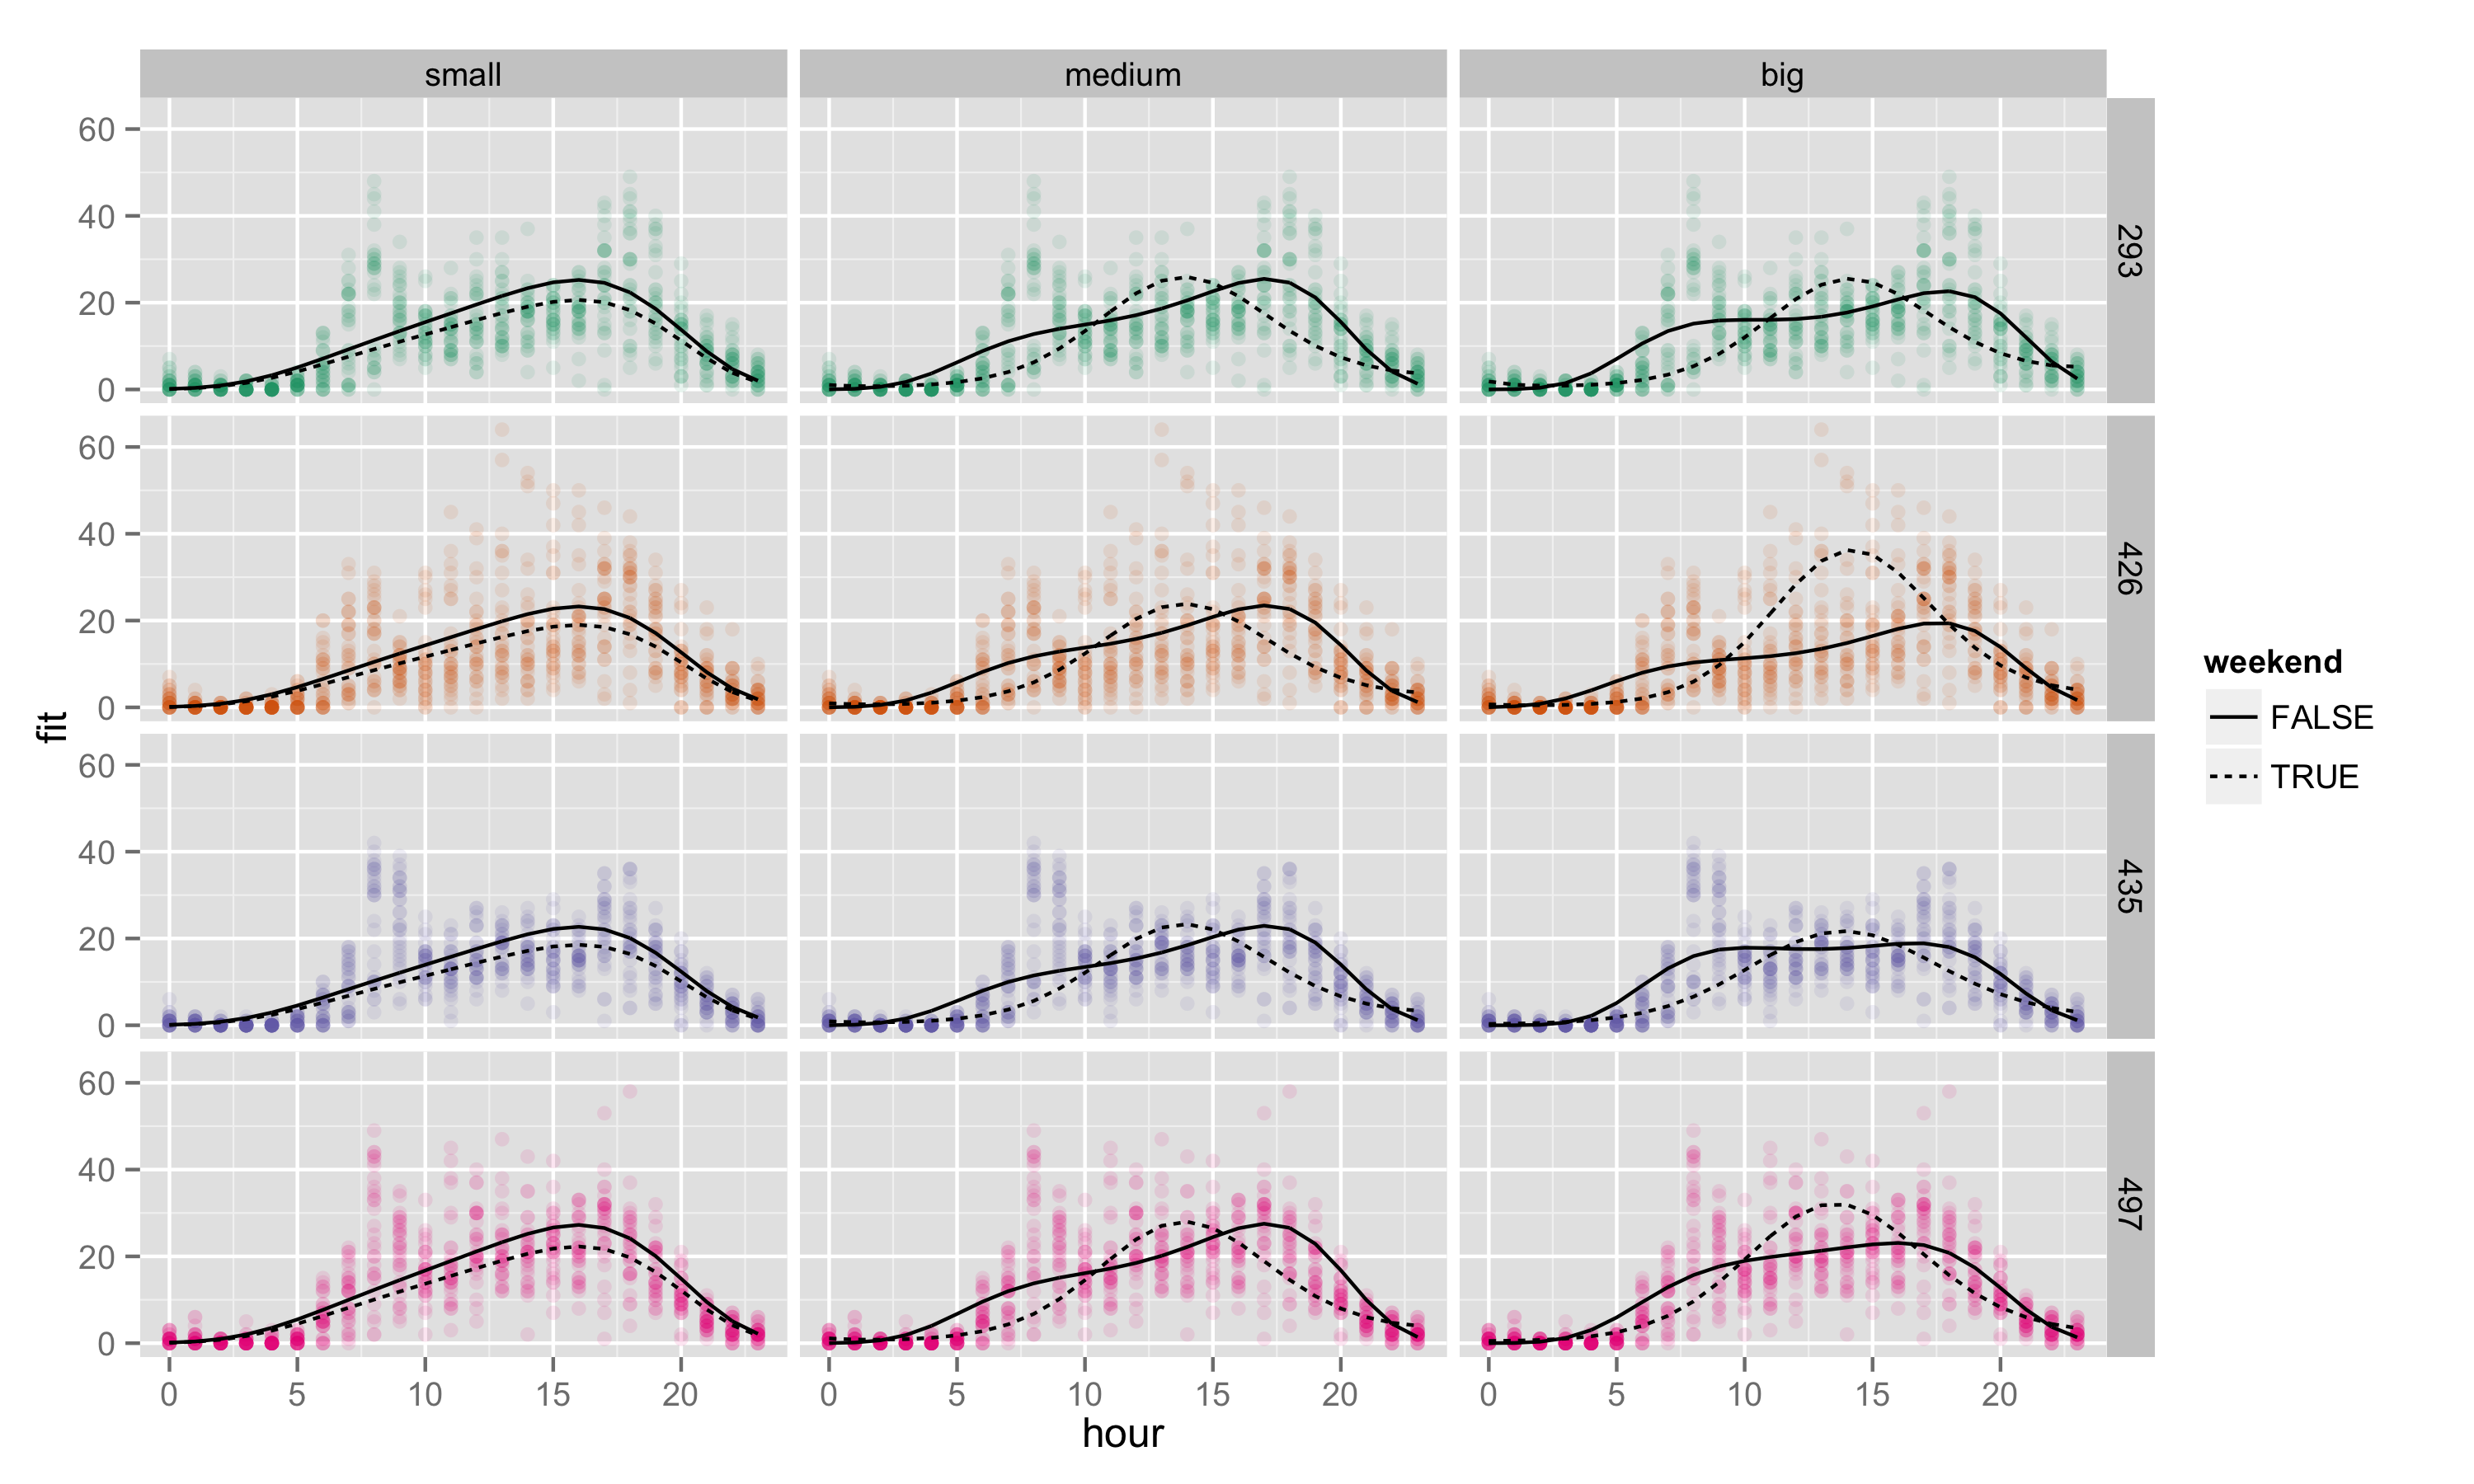
\includegraphics{./fig/fit_all.png}

\subsection{K-fold CV with a for loop}\label{k-fold-cv-with-a-for-loop}

Using a naive for loop, we could implement this as:

\begin{Shaded}
\begin{Highlighting}[]
\NormalTok{err.for <-}\StringTok{ }\OtherTok{NULL}
\KeywordTok{system.time}\NormalTok{(}
    \NormalTok{for (i in }\DecValTok{1}\NormalTok{:K) \{}
        \NormalTok{err.for <-}\StringTok{ }\KeywordTok{cbind}\NormalTok{(err.for, }\KeywordTok{get.errs}\NormalTok{(}\DataTypeTok{test.set =} \NormalTok{cv.test.sets[, i],}
                                           \DataTypeTok{discarded =} \NormalTok{discarded,}
                                           \DataTypeTok{q =} \DecValTok{1}\NormalTok{))}
        \NormalTok{\}}
    \NormalTok{)}
\end{Highlighting}
\end{Shaded}

\begin{verbatim}
##    user  system elapsed 
##  14.132   0.732  14.902
\end{verbatim}

\subsection{K-fold CV with an apply
function}\label{k-fold-cv-with-an-apply-function}

If you're good with \texttt{apply()} functions you might upgrade
(slightly) to

\begin{Shaded}
\begin{Highlighting}[]
\NormalTok{## apply version}
\KeywordTok{system.time}\NormalTok{(}
    \NormalTok{err.apply <-}\StringTok{ }\KeywordTok{sapply}\NormalTok{(}\DataTypeTok{X =} \DecValTok{1}\NormalTok{:K, }
                        \DataTypeTok{FUN =} \NormalTok{function(i) \{}
                            \KeywordTok{get.errs}\NormalTok{(}\DataTypeTok{test.set =} \NormalTok{cv.test.sets[, i],}
                                     \DataTypeTok{discarded =} \NormalTok{discarded,}
                                     \DataTypeTok{q =} \DecValTok{1}\NormalTok{)}
                            \NormalTok{\}}
                        \NormalTok{)}
    \NormalTok{)}
\end{Highlighting}
\end{Shaded}

\begin{verbatim}
##    user  system elapsed 
##  13.847   0.680  14.551
\end{verbatim}

Neither of the first two methods take advantage of multiple processors.
While the \texttt{apply()} functions avoid the inherently sluggish
nature of for loops in \texttt{R}, they are still ignorant of the
processor structure. We want to chop the job into halves, fourths, etc.
and use the \emph{whole} computer!

\subsection{K-fold CV with a snowfall
loop}\label{k-fold-cv-with-a-snowfall-loop}

Here is the same computation written with a \texttt{snowfall} loop

\begin{Shaded}
\begin{Highlighting}[]
\NormalTok{## Define a wrapper function}
\NormalTok{wrapper =}\StringTok{ }\NormalTok{function(i)\{}
  \KeywordTok{get.errs}\NormalTok{(}\DataTypeTok{test.set =} \NormalTok{cv.test.sets[, i], }\DataTypeTok{discarded =} \NormalTok{discarded, }\DataTypeTok{q =} \DecValTok{1}\NormalTok{)}
\NormalTok{\}}

\NormalTok{## snowfall version}
\KeywordTok{library}\NormalTok{(snowfall)}
\KeywordTok{library}\NormalTok{(parallel)}
\KeywordTok{library}\NormalTok{(rlecuyer)}
\CommentTok{# ## determines the number of cores on the machine}
\NormalTok{cps=}\KeywordTok{detectCores}\NormalTok{()}
\NormalTok{## Initalize multicore }
\KeywordTok{sfInit}\NormalTok{(}\DataTypeTok{parallel=}\OtherTok{TRUE}\NormalTok{, }\DataTypeTok{cpus=}\NormalTok{cps)}
\NormalTok{## Setup random number generator on the cluster}
\KeywordTok{sfClusterSetupRNG}\NormalTok{()}
\CommentTok{# export global variables}
\KeywordTok{sfExportAll}\NormalTok{()}
\CommentTok{# export library}
\KeywordTok{sfLibrary}\NormalTok{(splines)}
\KeywordTok{system.time}\NormalTok{(err.snowfall <-}\StringTok{ }\KeywordTok{sfSapply}\NormalTok{(}\DecValTok{1}\NormalTok{:K, wrapper))}
\NormalTok{## ends snowfall session}
\KeywordTok{sfStop}\NormalTok{()}
\end{Highlighting}
\end{Shaded}

\section{components of a snowfall
loop}\label{components-of-a-snowfall-loop}

Note that the syntax of snowfall is almost identical to a for loop. The
major difference is the need to write a wrapper function that evaluates
one iteration of the for loop and the need to set up and export the
relevent data, functions, and libraries.

\section{results}\label{results}

\href{http://CRAN.R-project.org/package=snowfall}{snowfall}

\subsection{Other tutorials}\label{other-tutorials}

\subsection{Data}\label{data-1}

\href{https://www.citibikenyc.com/system-data}{citibike system data}

\end{document}
